
\begin{enumerate}
    \item \textbf{Kratak opis:} Nakon primanja zahteva od strane korisnika, sistem obrad1uje zahtev, odred1ivanjem rute, vozacha i vozila. Na osnovu ovih podataka izrachunava se i ochekivano vremene pristizanja robe, kao i procena cene transporta.
    
    \item \textbf{Uchesnici:} Sistem, Korisnik, Vozach, Magacioner, Logistichar.
    \item \textbf{Preduslovi:}  Sistem je u funkciji. Korisnik je poslao zahtev za transport koji je zabelezhen u sistemu.
    
    \item \textbf{Postuslovi:} Zahtev je obrađen. U sistemu su zabelezhene sve informacije.
    \item \textbf{Osnovni tok:}
        \begin{enumerate}
            \item[5.1.] Iz baze podataka se chitaju informacije dostavljenje od strane korisnika prilikom slanja zahteva.
            
            \item[5.2.] Vrshi se odred1ivanje rute, opisano u podtoku P1.
            \item[5.3.] Vrshi se dodela vozila, opisano u podtoku P2.
            \item[5.4.] Vrshi se dodela vozacha, opisano u podtoku P3.
            \item[5.5.] Na osnovu informacija o ruti i vozilu koje je dodeljeno se odred1uje vreme pristizanja poshiljke i cena.
            \item [5.6.] Informacije o procenjenoj ceni i vremenu se chuvaju u sistemu.
            \item [5.7.] Izveshtaj o uspeshnoj obradi zahteva se shalje Logisticharu.
            \item [5.8.] Izveshtaj o uspeshnoj obradi zahteva se shalje Korisniku.
            \item [5.9.] Izveshtaj o narud2bini shalje svakom od vozacha.
            \item [5.10.] Izveshtaj o narud2bini se shalje Magacioneru.
        \end{enumerate}
    \item \textbf{Alternativni tokovi:}
            \begin{itemize}
            
            \item [A1.] Ukoliko u koraku 5.3. ne postoje dostupna vozila. 
            U sistemu se chuva informacija da je obrada zahteva na chekanju. Logisticharu se shalje izveshtaj o neuspeloj dodeli vozila. Nakon shto se u sistemu zabelezhi da postoje slobodna vozila, nastavlja se od koraka 5.3.
            
            \item [A2.] Ukoliko u koraku 5.4. nema dovoljan broj vozacha 
            U sistemu se chuva informacija da je obrada zahteva na chekanju. Logisticharu se shalje izveshtaj o neuspeloj dodeli vozila. Nakon shto se u sistemu zabelezhi da postoje slobodna vozachi, nastavlja se od koraka 5.4.
            
            \end{itemize}
        
    \item \textbf{Podtokovi:} 
            \begin{itemize}
                \item \textbf{P\-1. Odred1ivanje rute}
                \begin{enumerate}
                    \item Iz baze podataka se chitaju informacije o adresi dostave.
                    \item Odred1uje se ruta.
                    \item Ruta se belezhi u sistemu.
                \end{enumerate}
                
                \item \textbf{P\-2. Odred1ivanje vozila}
                \begin{enumerate}
                    \item Iz baze podataka se chitaju informacije o zahtevanoj kolichini robe.
                    \item Na osnovu dostupnih vozila i njihove nosivnosti, odred1uju se vozila za transport.
                    \item Informacije o rezervisanim vozilima se belezhi u sistem.
                \end{enumerate}
                
                \item \textbf{P\-3. Odred1ivanje vozacha}
                \begin{enumerate}
                    \item Iz baze se chitaju informacije o vozilima rezervisanim za transport.
                    \item Za svako vozilo se odred1uje vozach.
                    \item Informacije o vozachima koji vrshe transport se belezhe u sistem.
                \end{enumerate}
            \end{itemize}
    \item \textbf{Specijalni zahtevi:} /
    \item \textbf{Dodatne informacije:} 
            \begin{itemize}
                \item Izveshtaj koji se shalje Logisticharu sadrzhi sve prikupljene informacije. 
                \item Izveshtaj koji se shalje Korisniku sadrzhi informacije o naruchenoj kolichini shec1era, adresi dostave, kao i informacija o procenjenoj ceni i vremenu dostave.
                
                \item Izveshtaj koji se shalje svakom od Vozacha sadrzhi informacije o vozilu, adresi dostave.
                
                \item Izveshtaj koji se shalje Magacioneru sadrzhi informaciju o kolichini robe i vozilima.
                
                
            \end{itemize}
\end{enumerate}

\newpage

\begin{figure}[h!]
    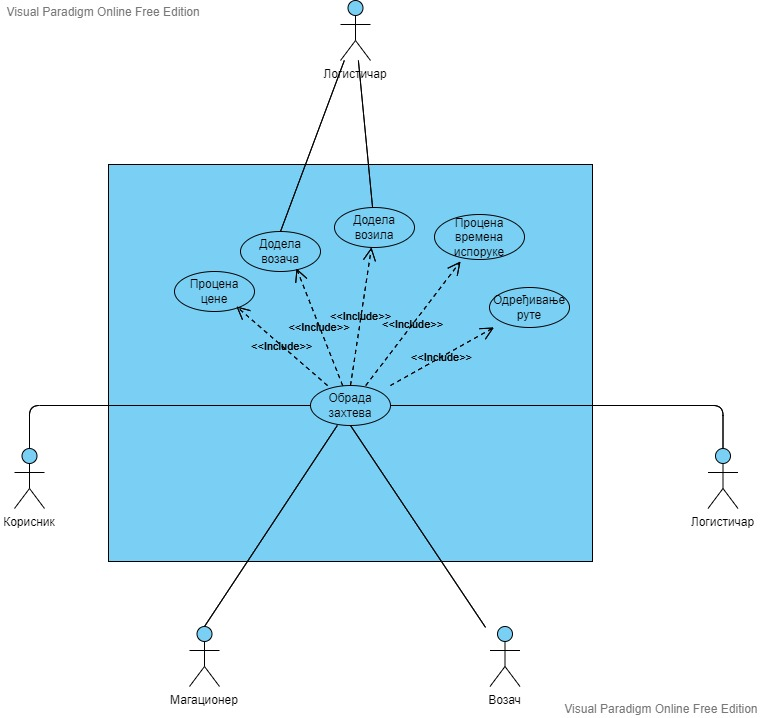
\includegraphics[scale=0.5]{Slike/UML/SUobrada.jpg}
    \centering
    \caption{Sluchaj upotrebe: Obrada poslatog zahteva za transport}
    \label{dsuobradazahteva}
\end{figure}    


